\begin{figure}[!htbp]
    {
%        \renewcommand{\arraystretch}{0.1}
        \setlength\tabcolsep{0em}
    	\centering	
    	\begin{tabular}{|p{5.3cm}p{5.3cm}p{5.3cm}|}
    		\hline
    		%		 
    		{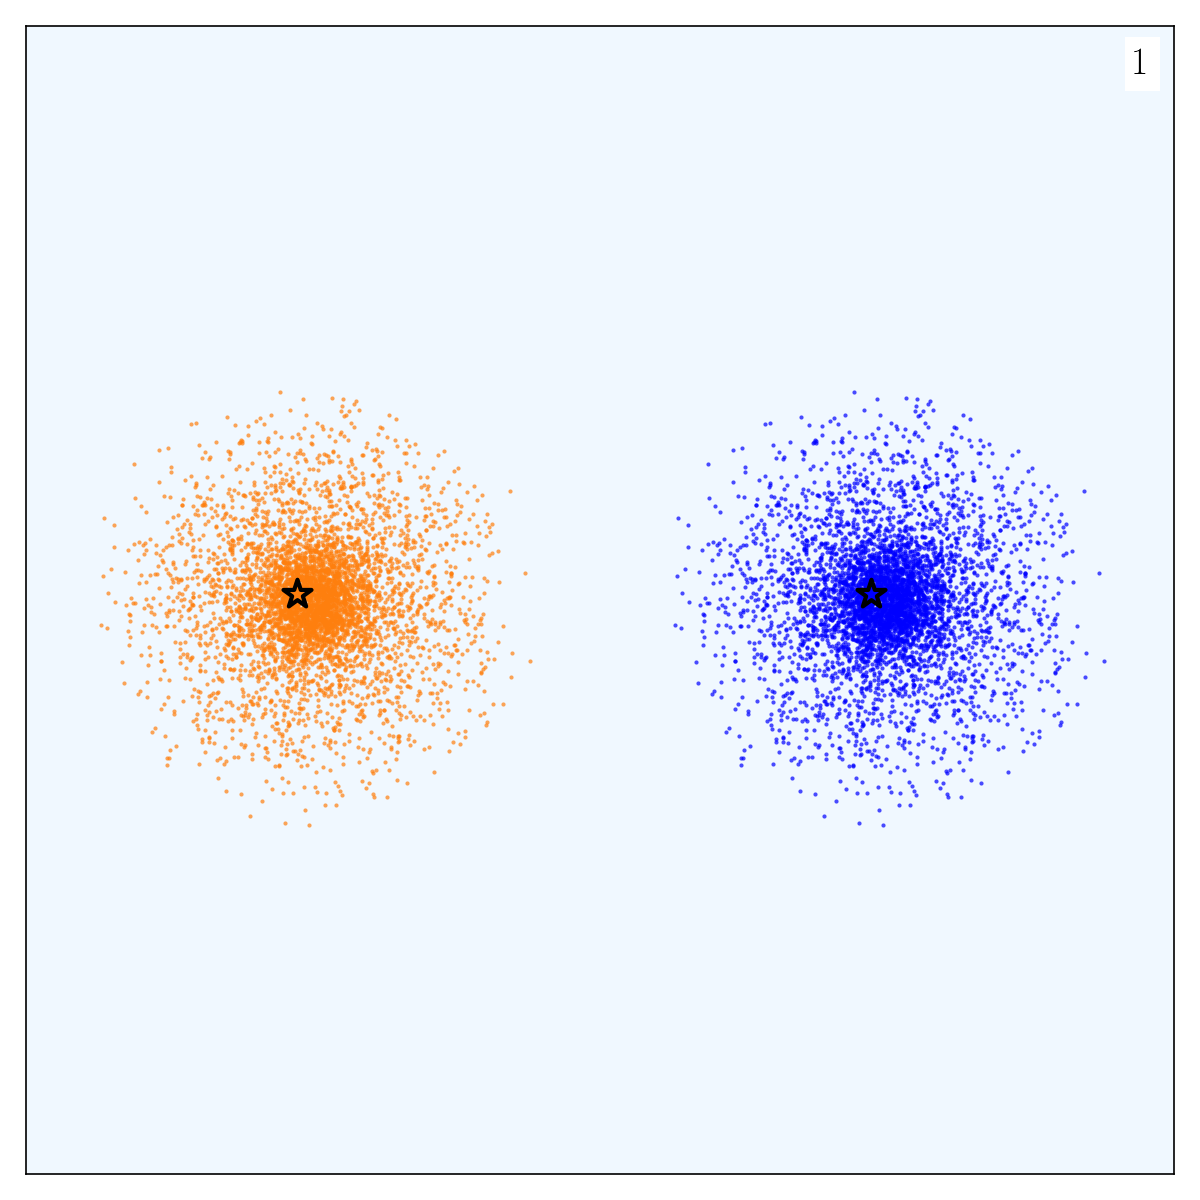
\includegraphics[width = 5.3cm]{images/jumper-demo/particleplot_00001.png}}	& 
    		{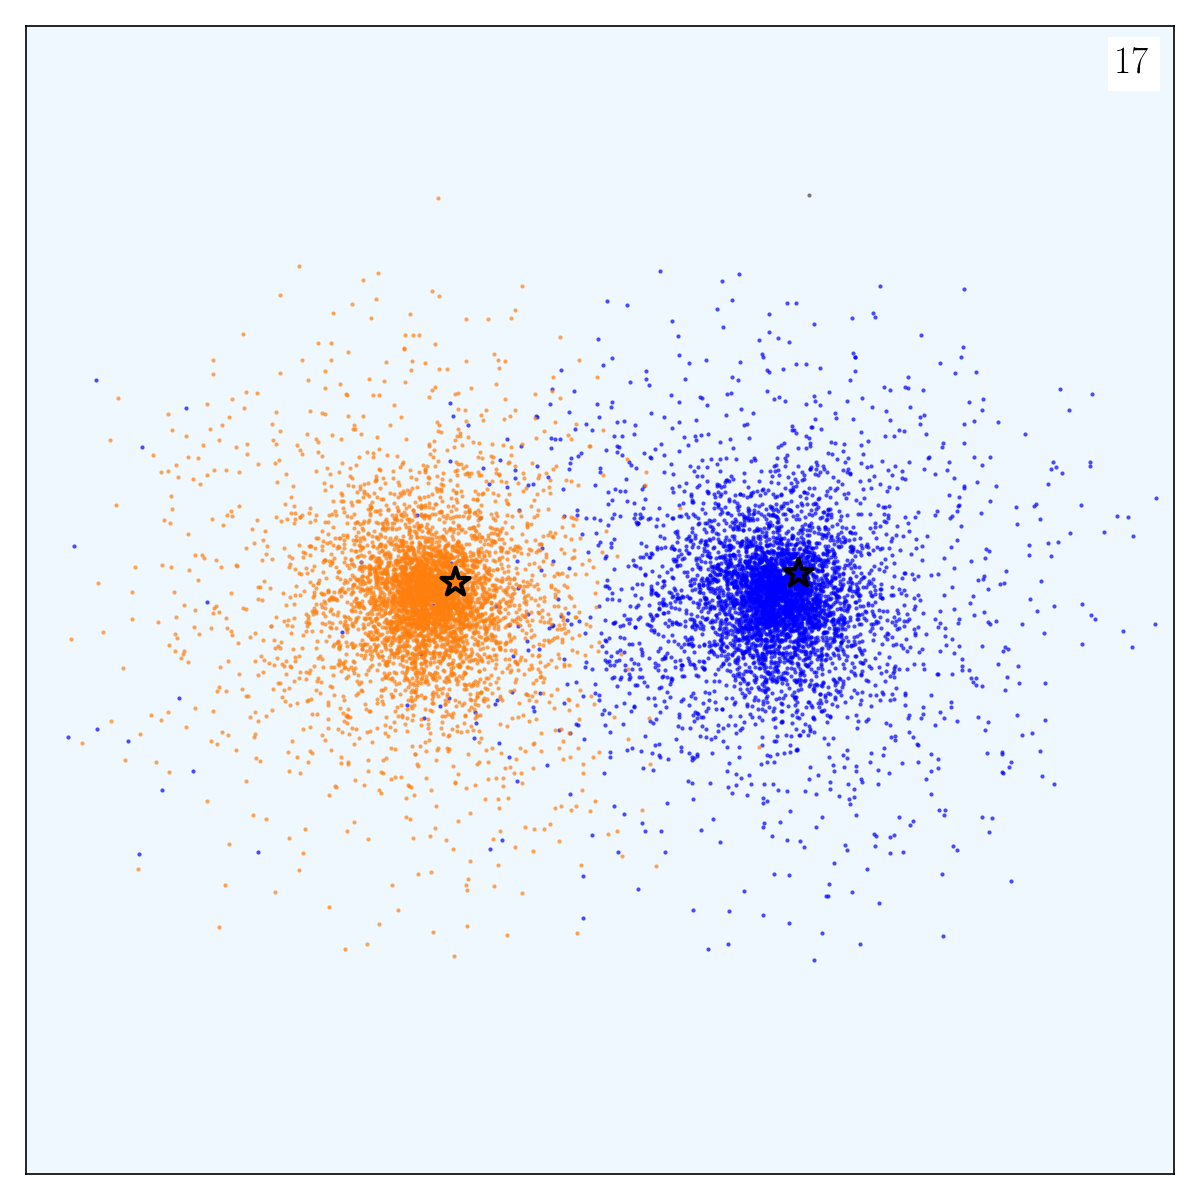
\includegraphics[width = 5.3cm]{images/jumper-demo/particleplot_00017.png}}	& 
    		{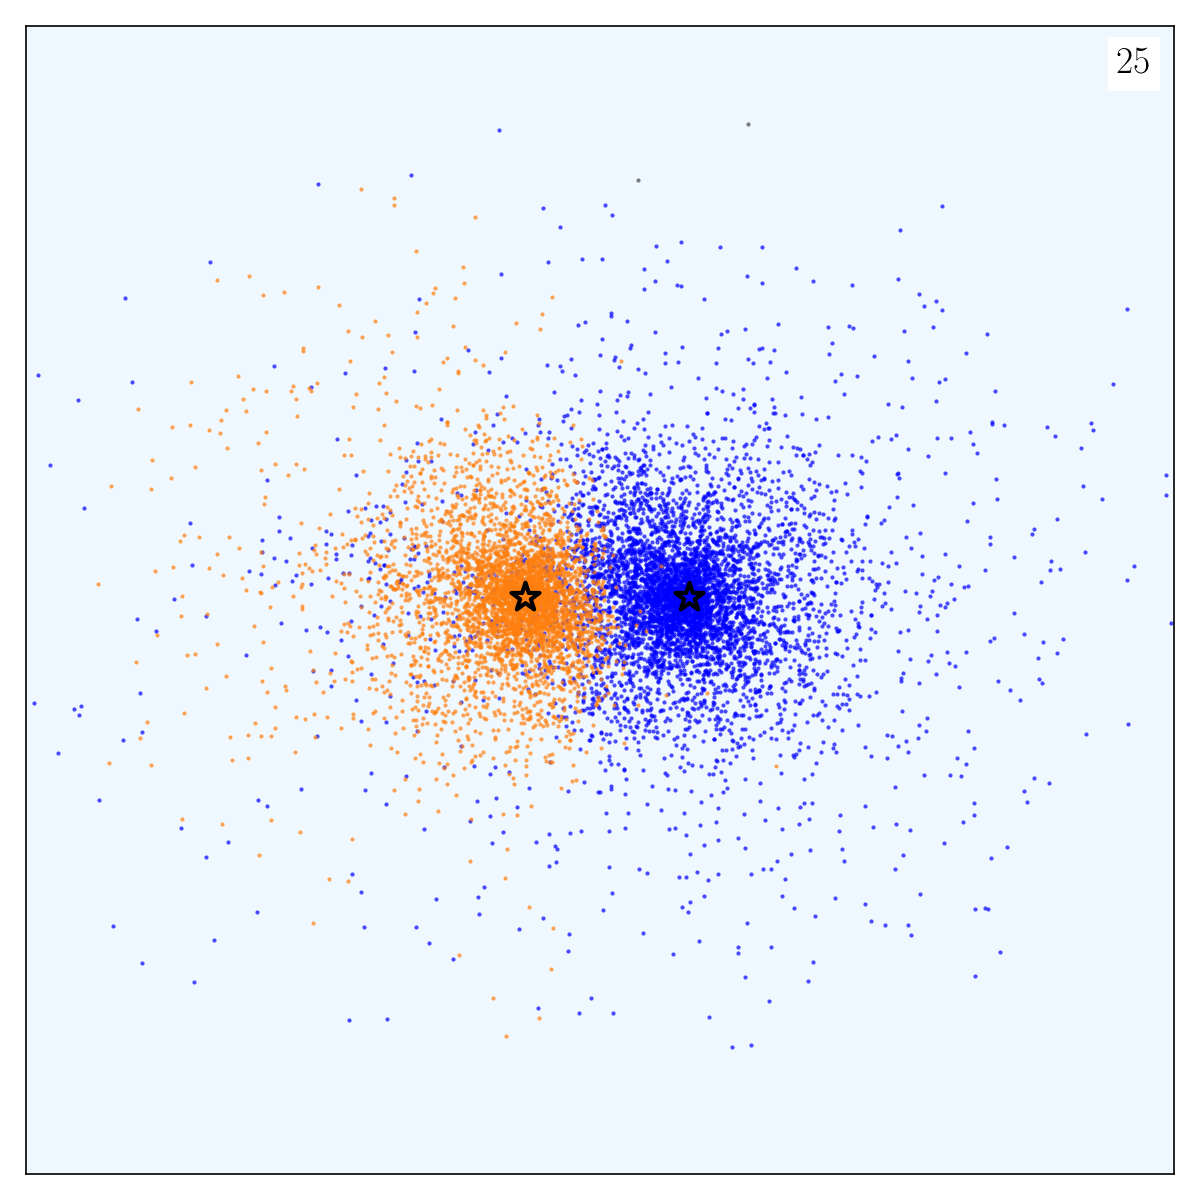
\includegraphics[width = 5.3cm]{images/jumper-demo/particleplot_00025.png}}  \\[-0.5em]
    		%
    		%
    		{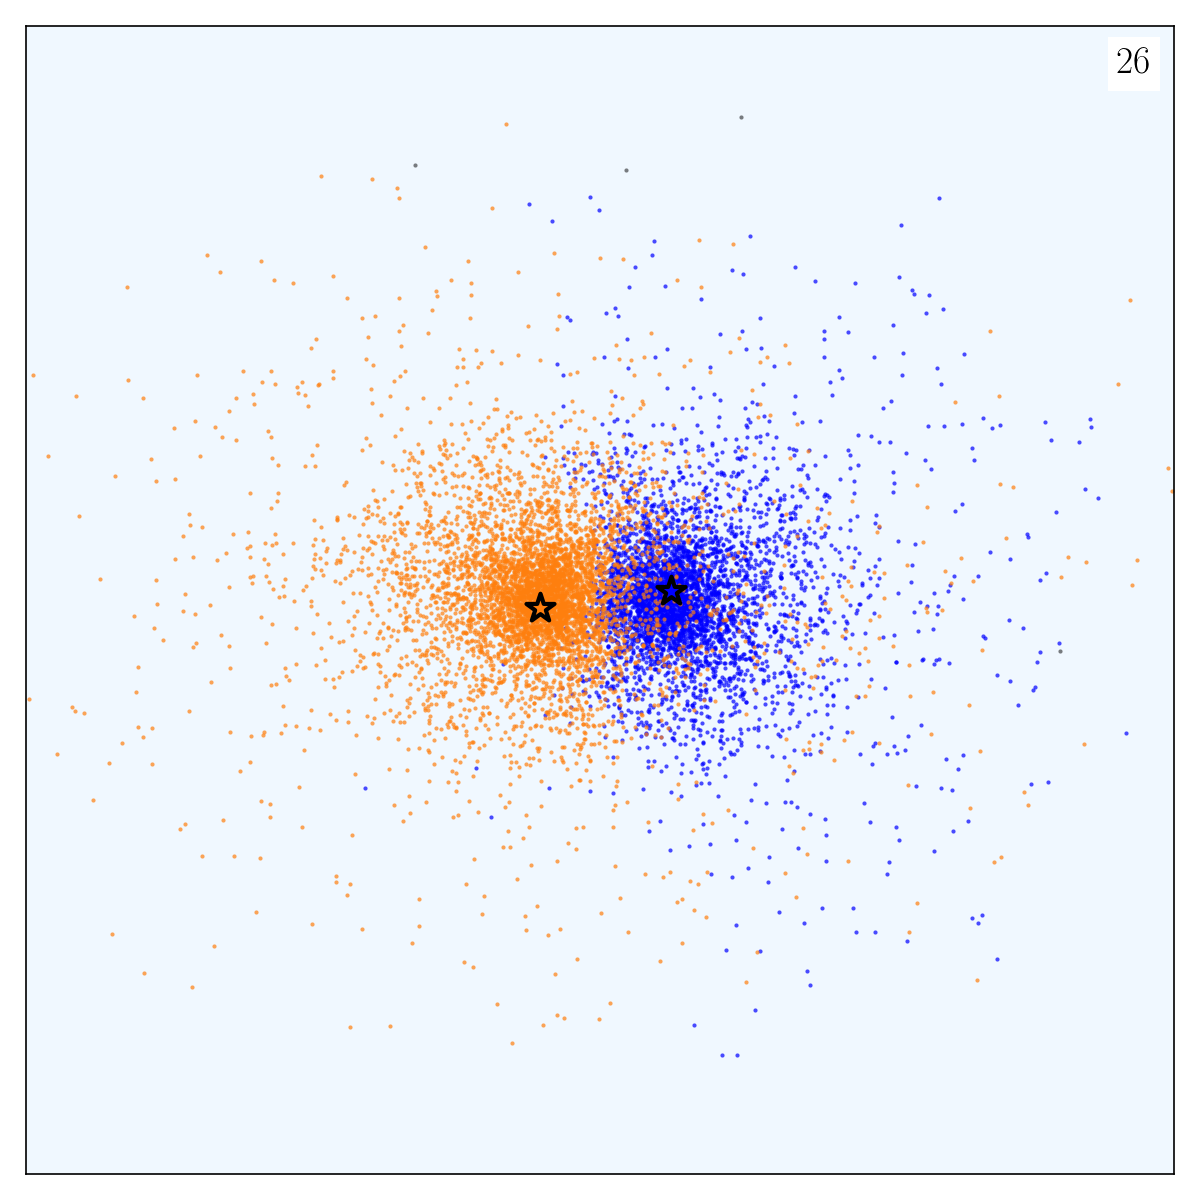
\includegraphics[width = 5.3cm]{images/jumper-demo/particleplot_00026.png}}	& 
    		{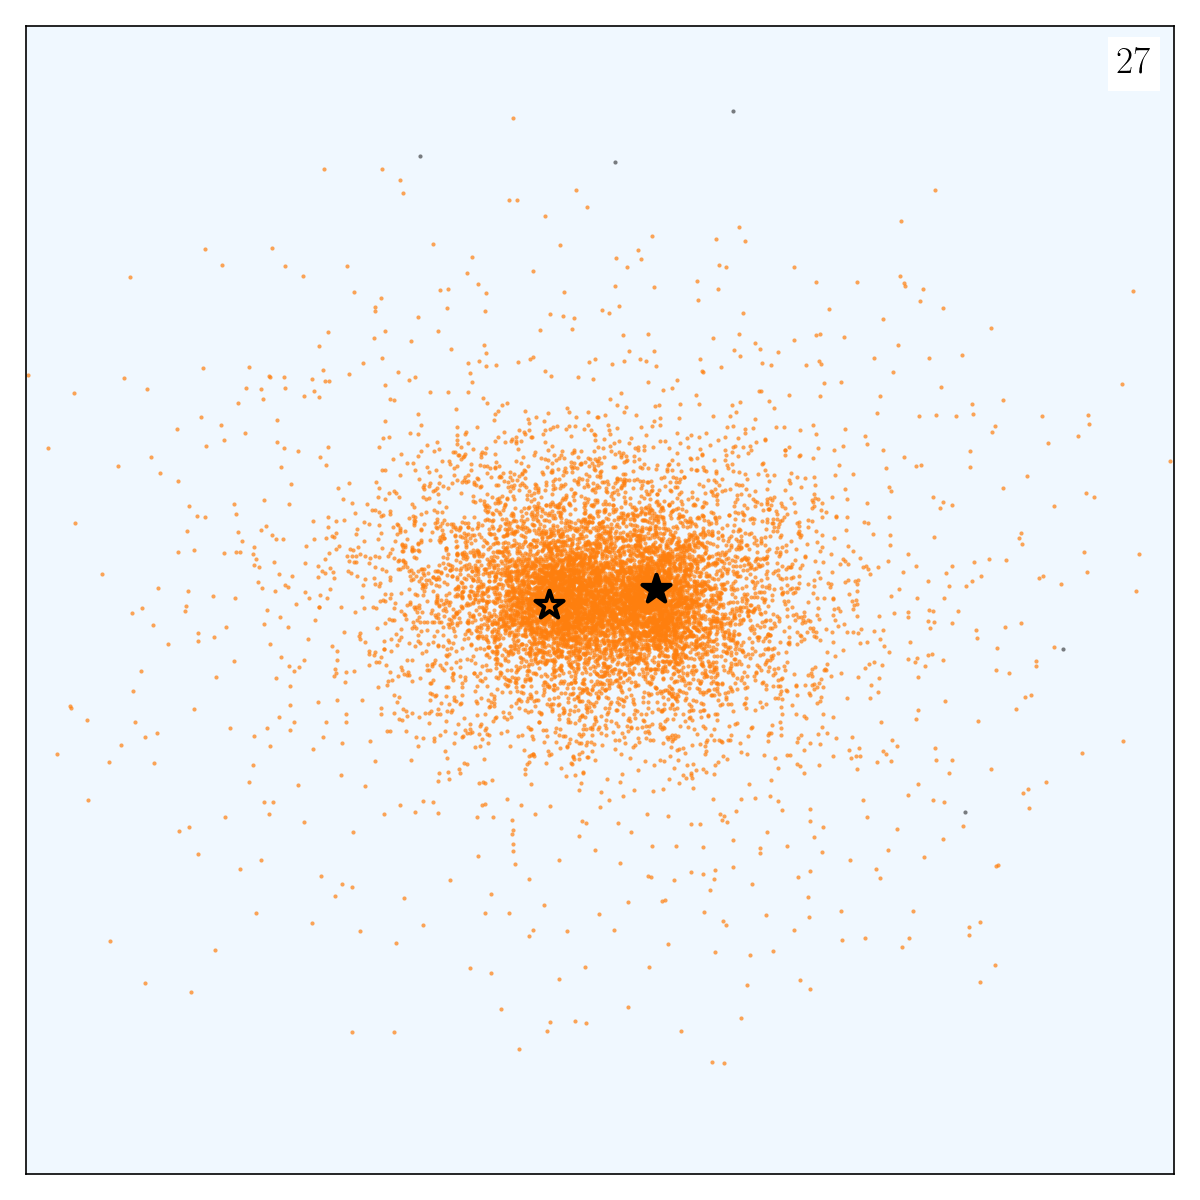
\includegraphics[width = 5.3cm]{images/jumper-demo/particleplot_00027.png}}	& 
            {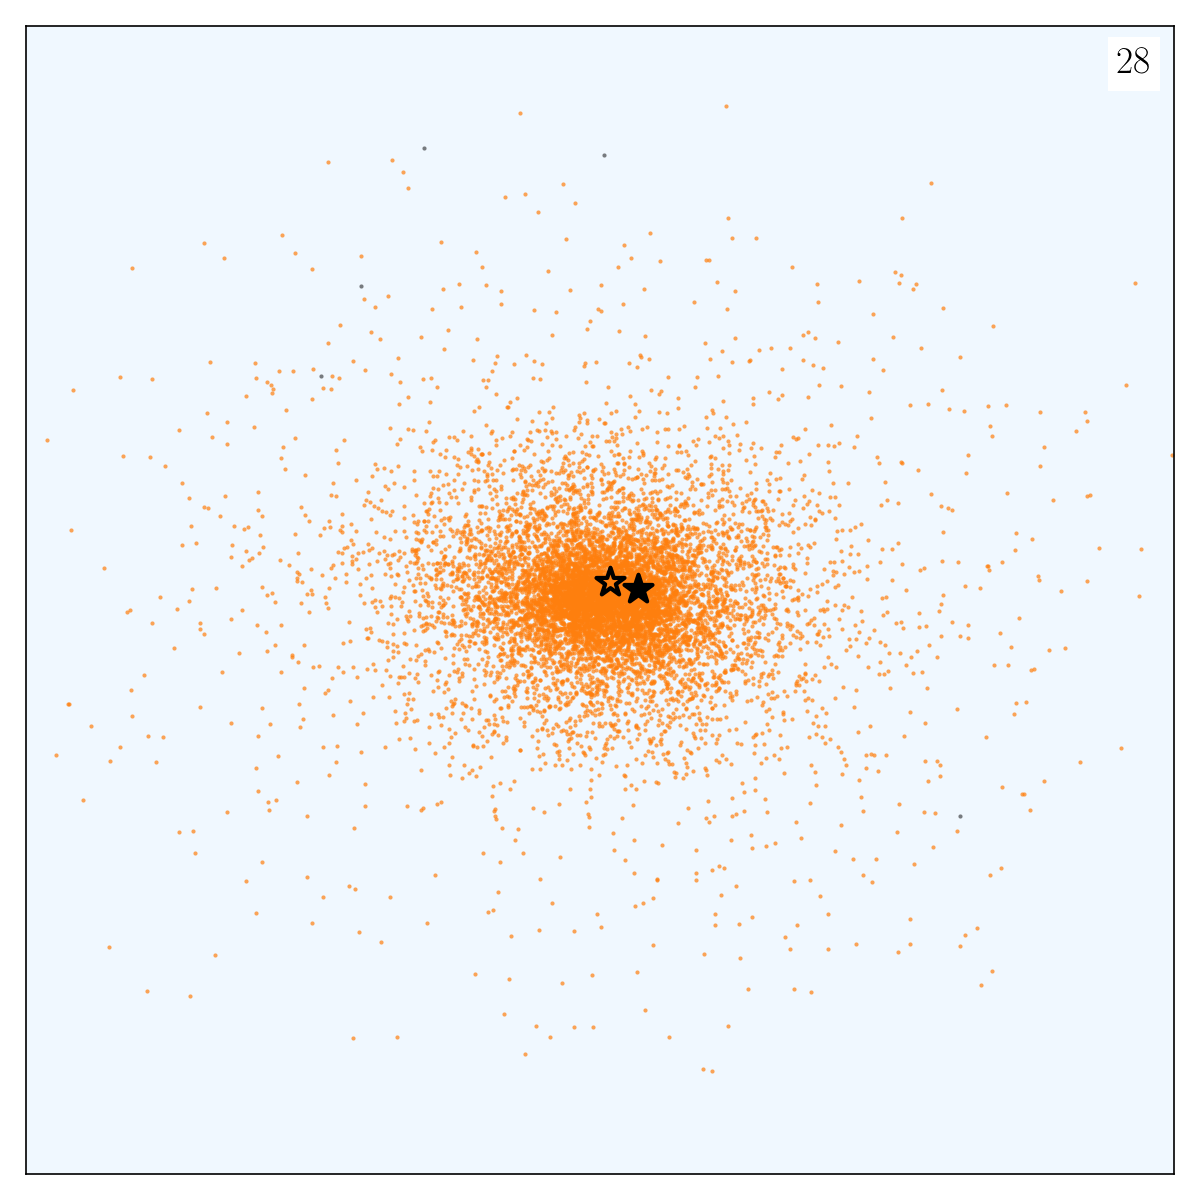
\includegraphics[width = 5.3cm]{images/jumper-demo/particleplot_00028.png}}	\\[-0.5em] 
    		%
            %
            {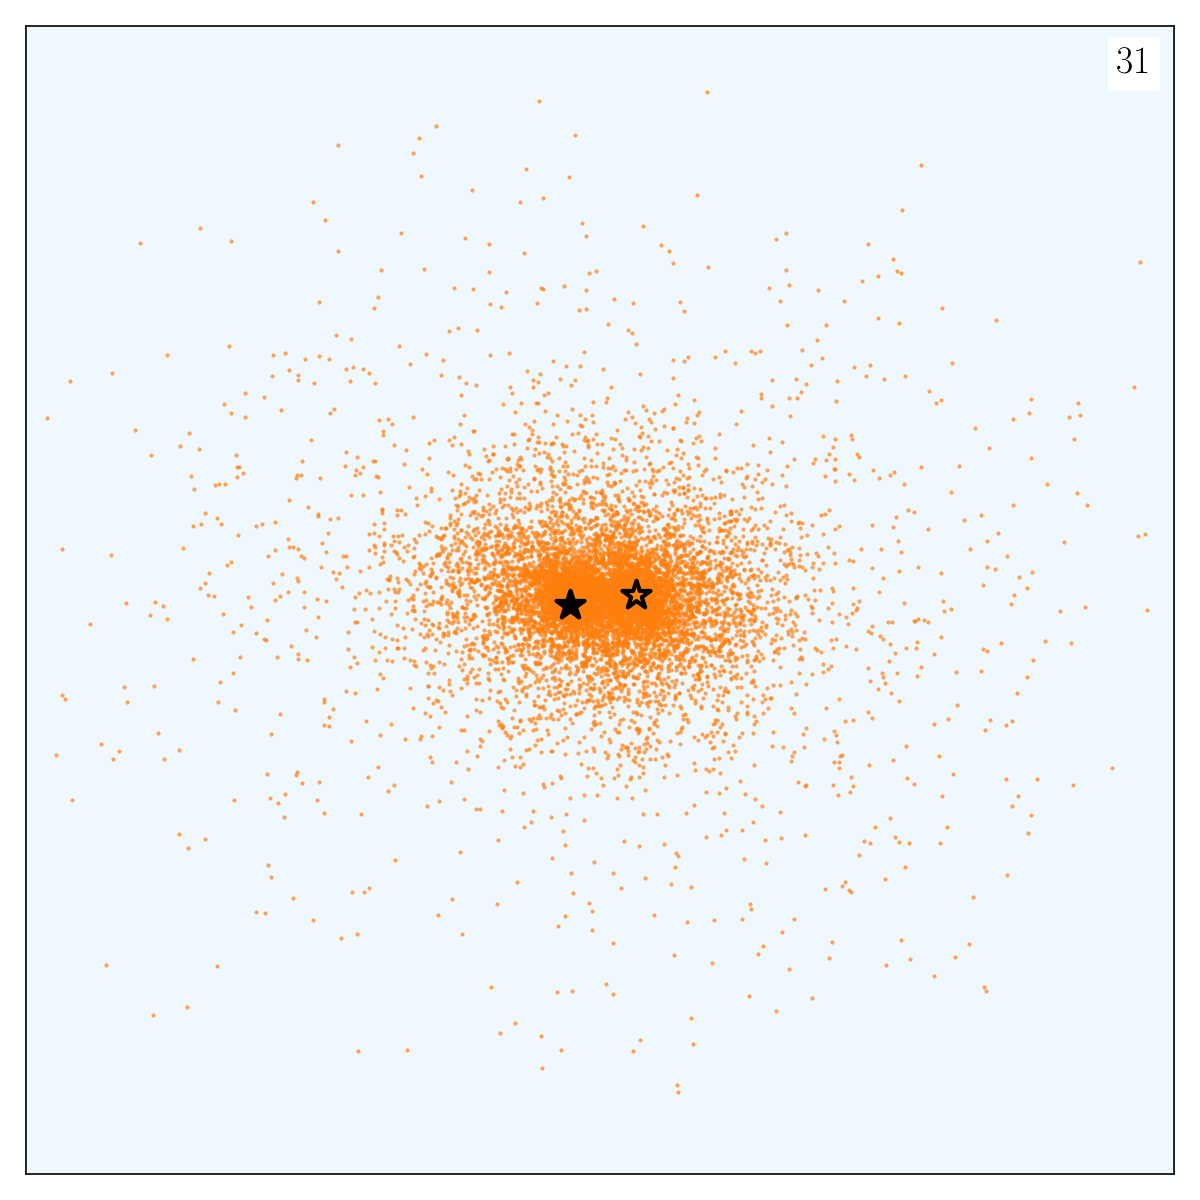
\includegraphics[width = 5.3cm]{images/jumper-demo/particleplot_00031.png}}    &
            {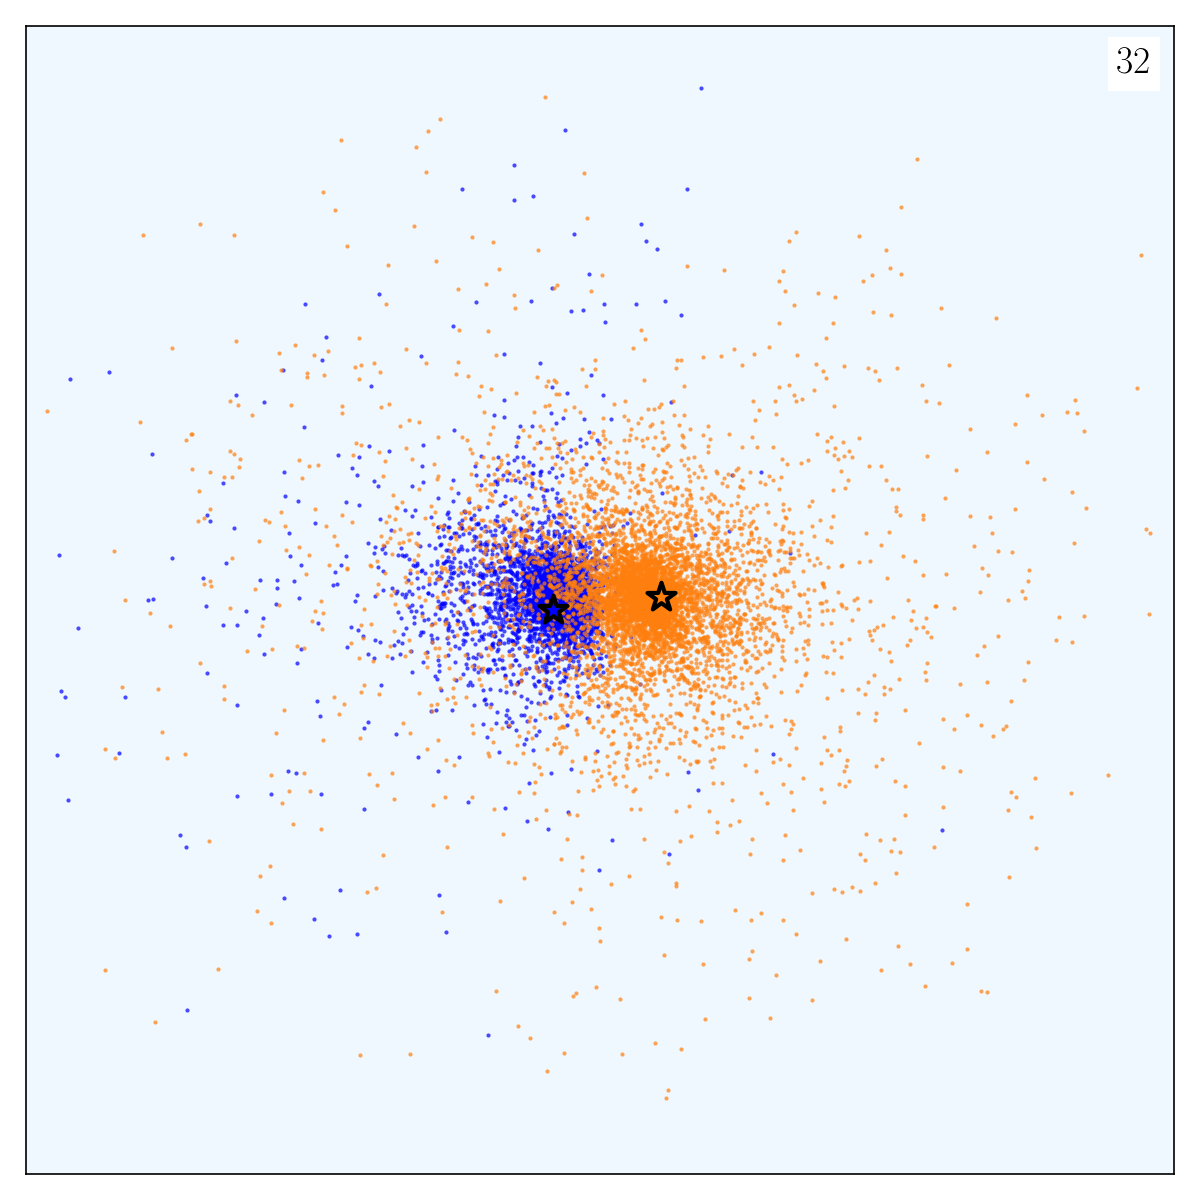
\includegraphics[width = 5.3cm]{images/jumper-demo/particleplot_00032.png}} 	&
            {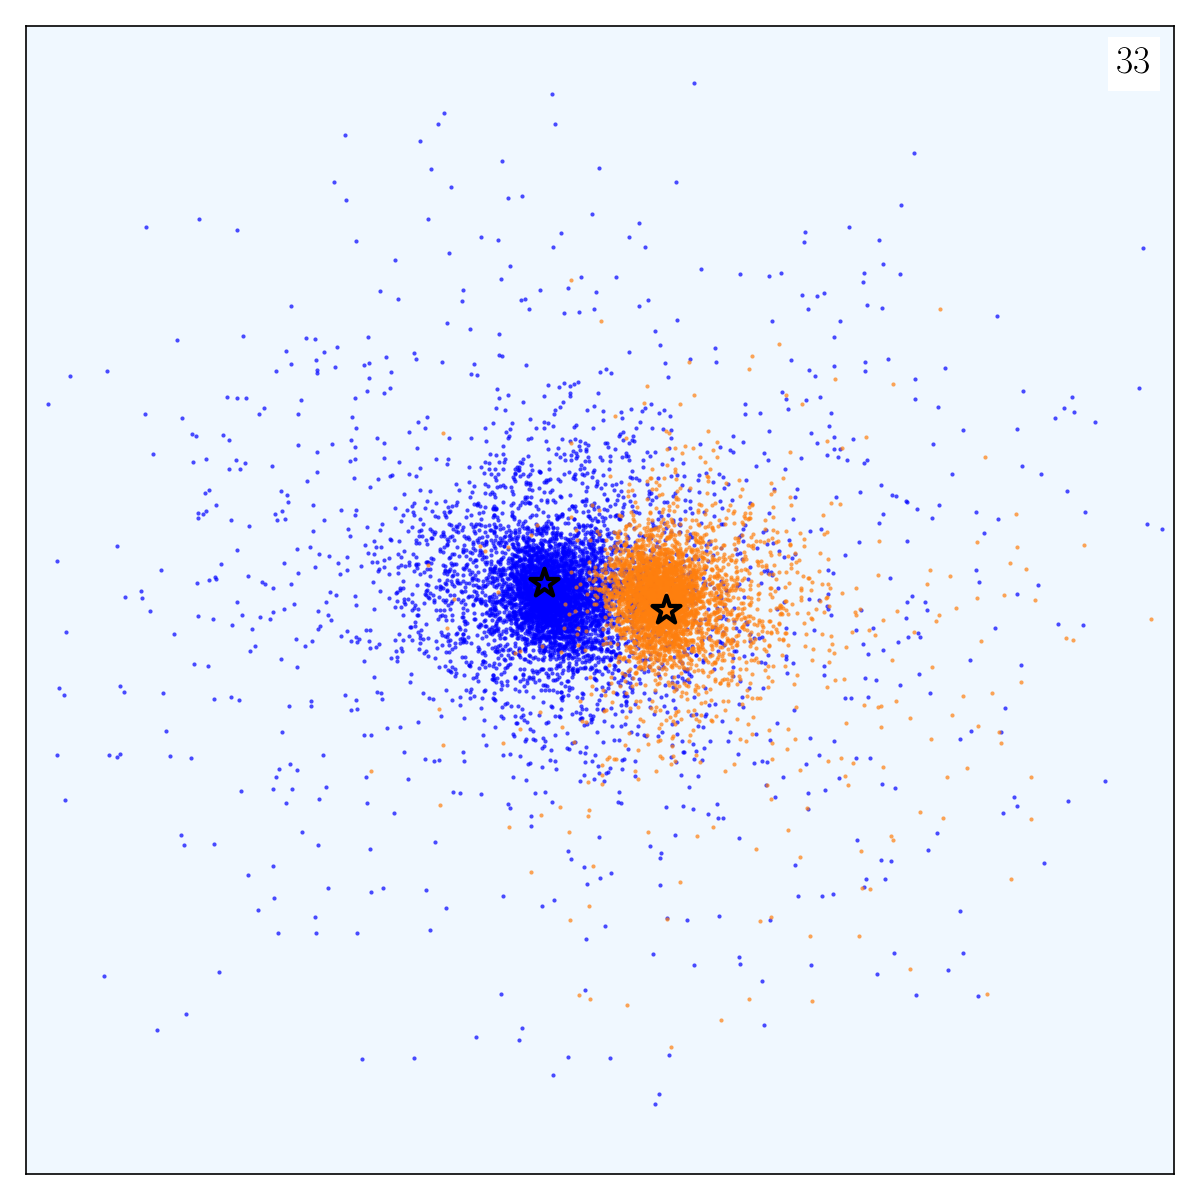
\includegraphics[width = 5.3cm]{images/jumper-demo/particleplot_00033.png}} 	\\[-0.5em]
    		%
            %
            {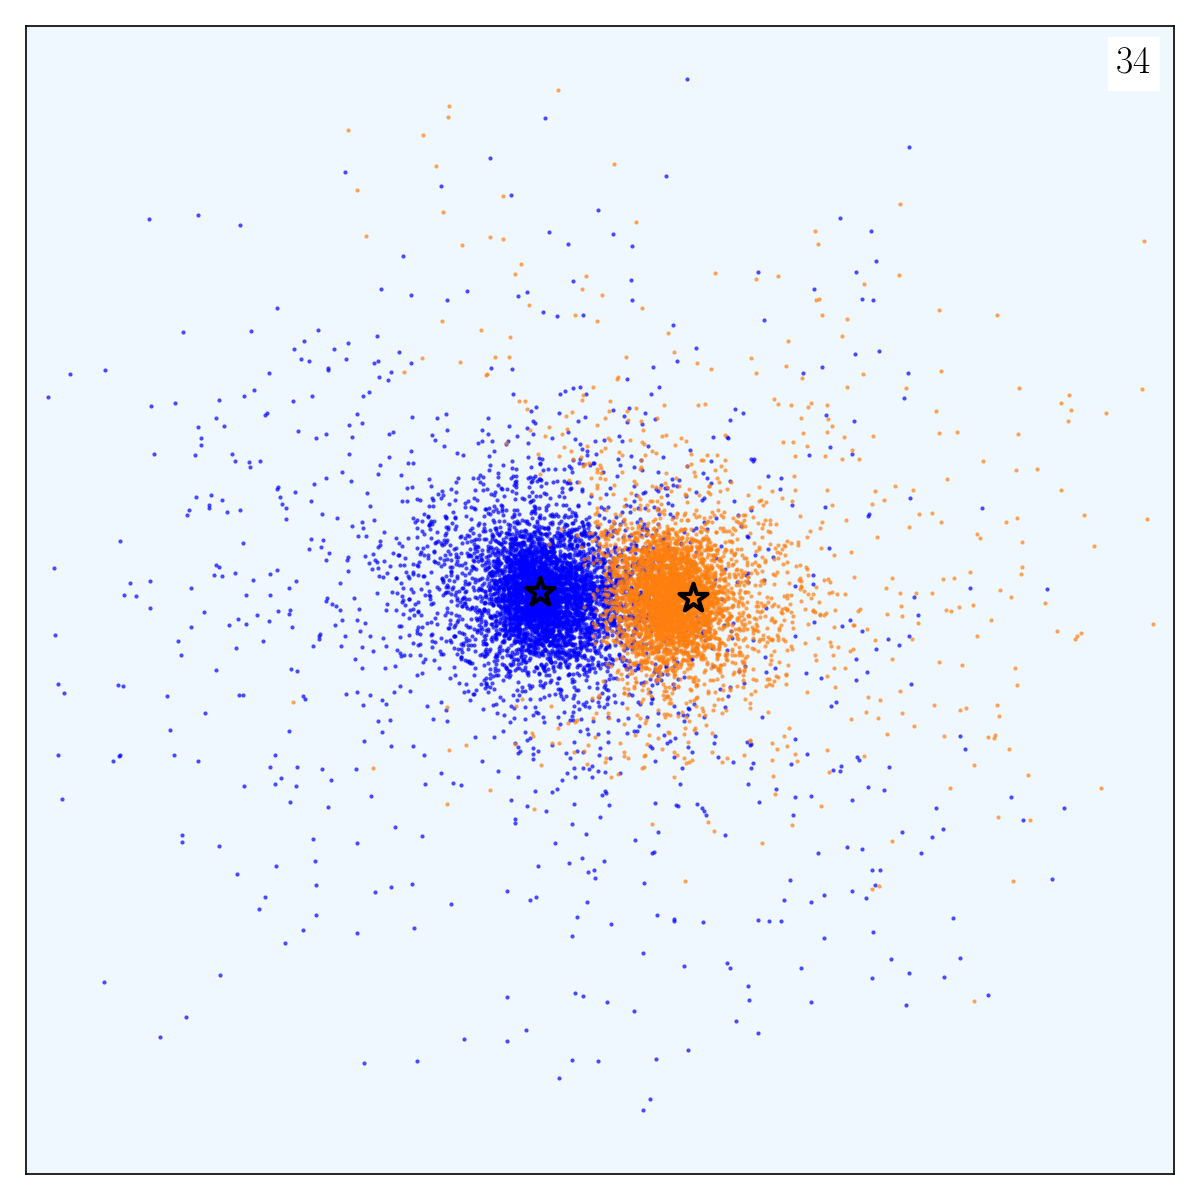
\includegraphics[width = 5.3cm]{images/jumper-demo/particleplot_00034.png}} 	& 
    		{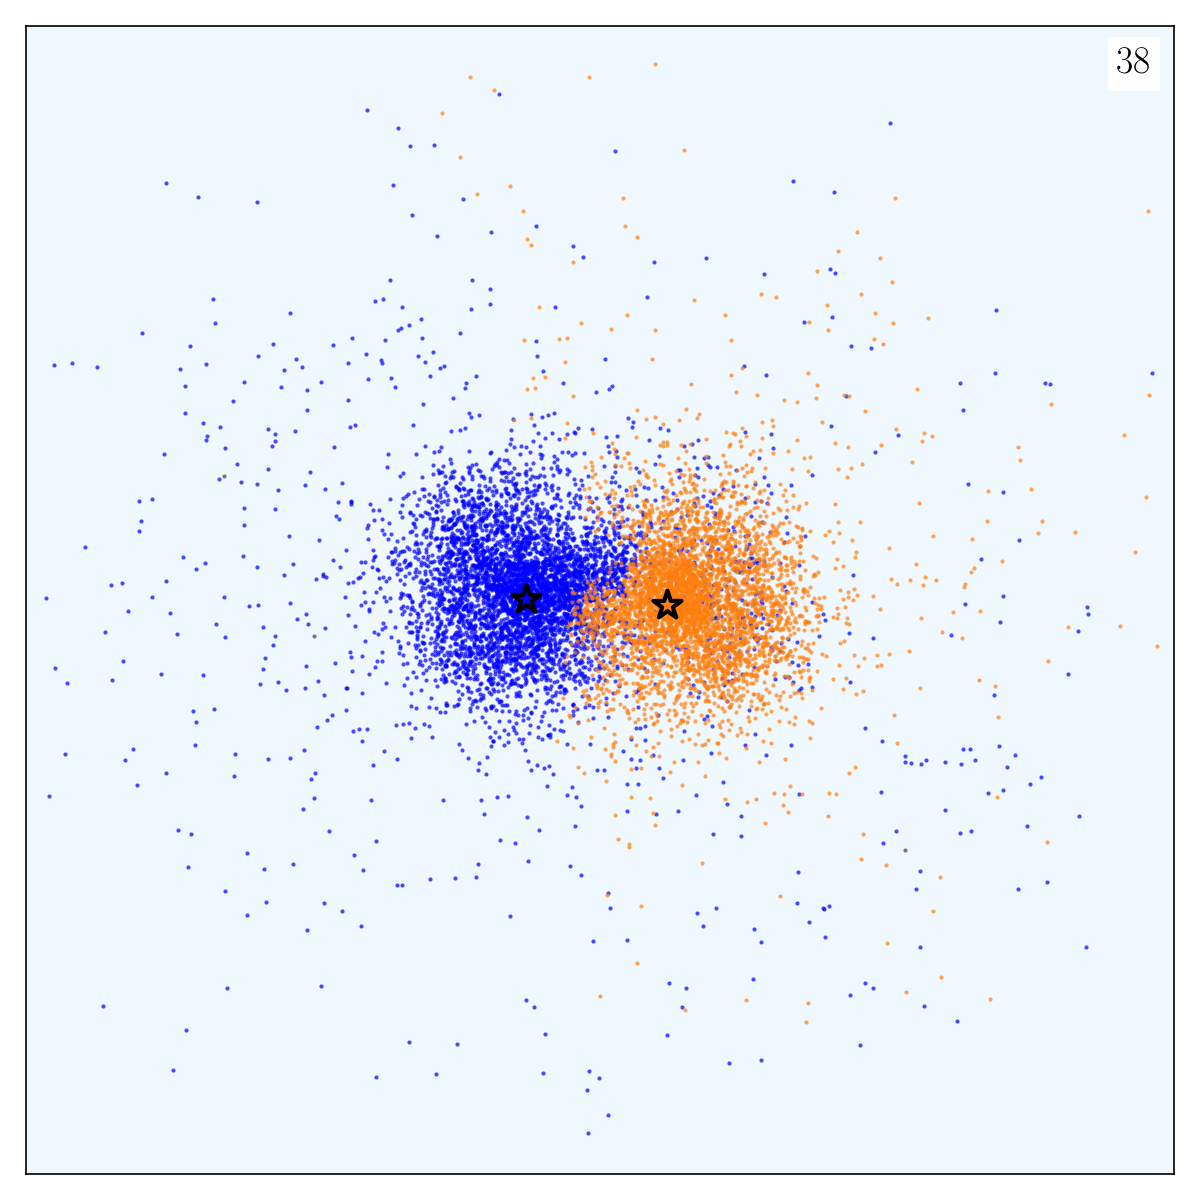
\includegraphics[width = 5.3cm]{images/jumper-demo/particleplot_00038.png}}	& 
            {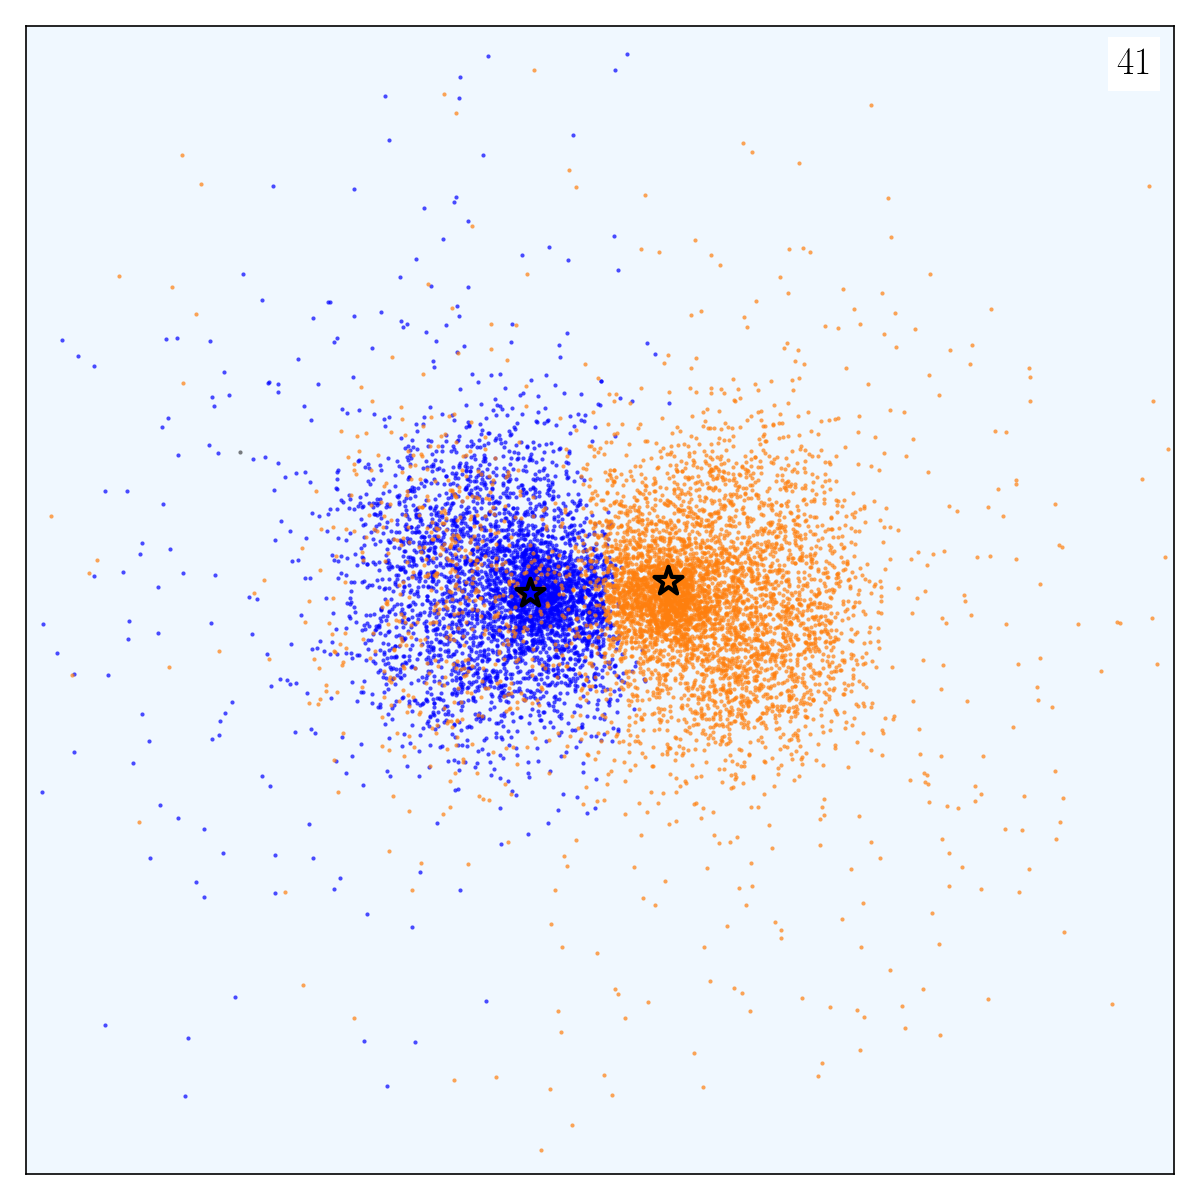
\includegraphics[width = 5.3cm]{images/jumper-demo/particleplot_00041.png}} 	\\%[-0.5em]
    		%
            %
%            {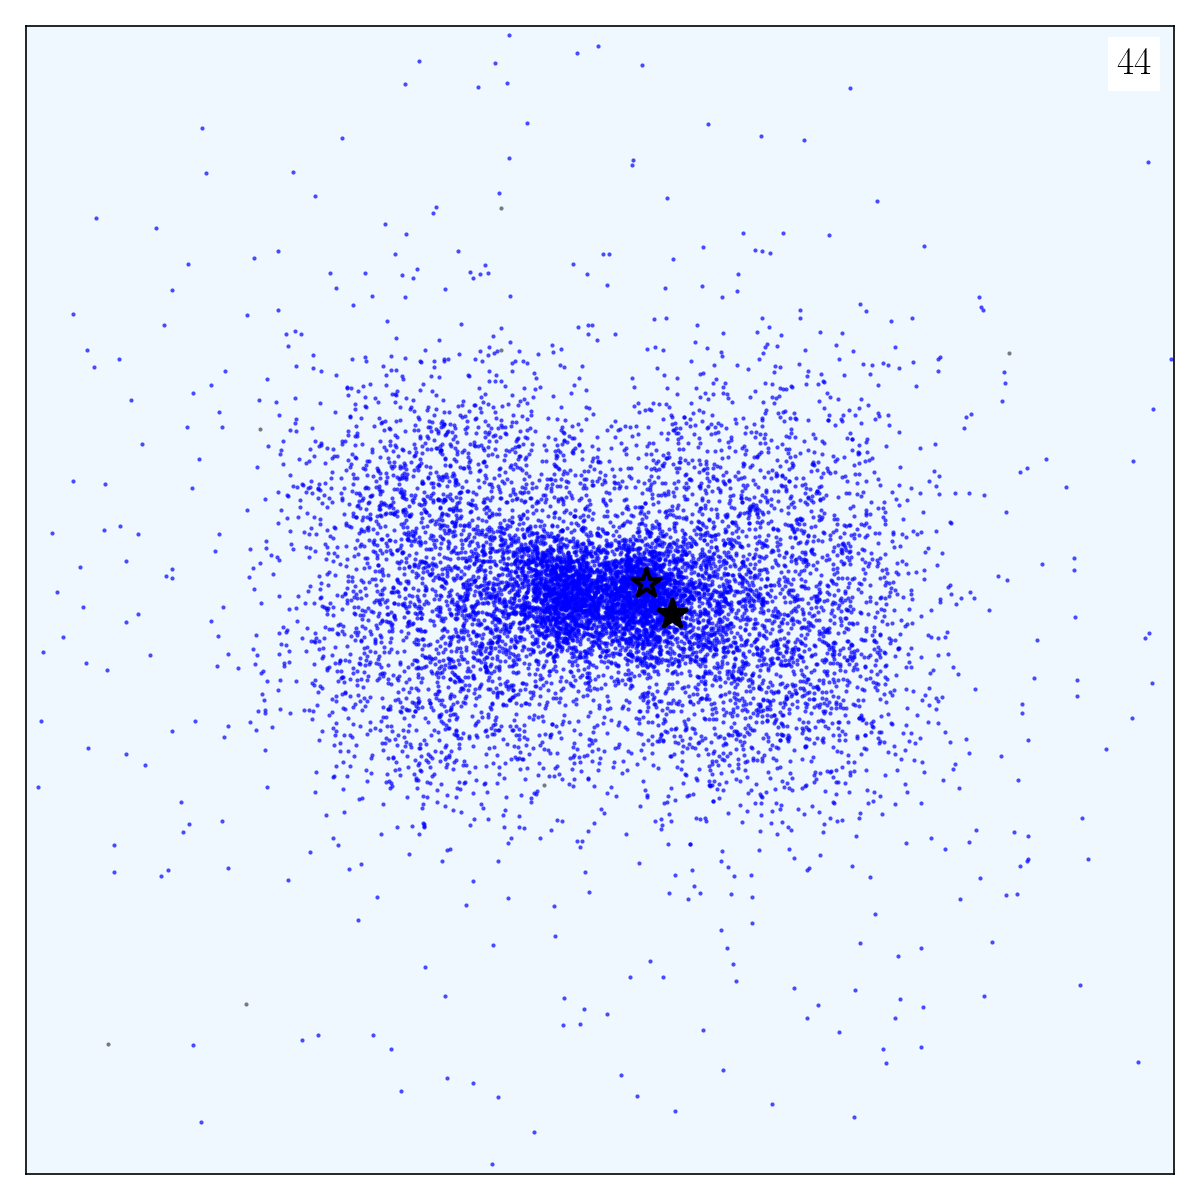
\includegraphics[width = 5.3cm]{images/jumper-demo/particleplot_00044.png}} 	& 
%    		{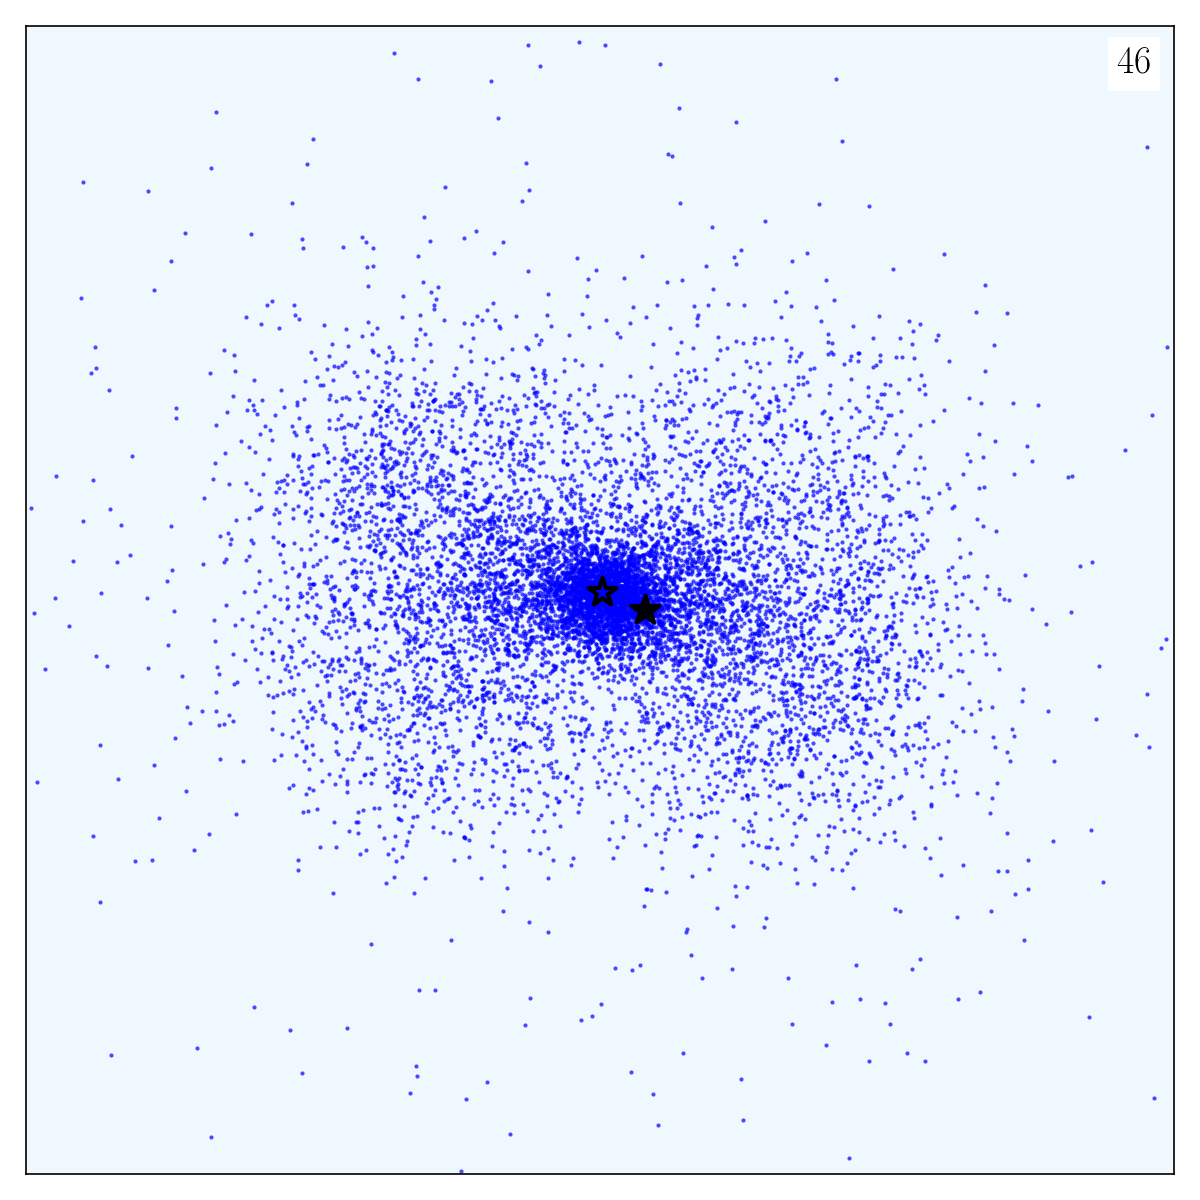
\includegraphics[width = 5.3cm]{images/jumper-demo/particleplot_00046.png}}	& 
%            {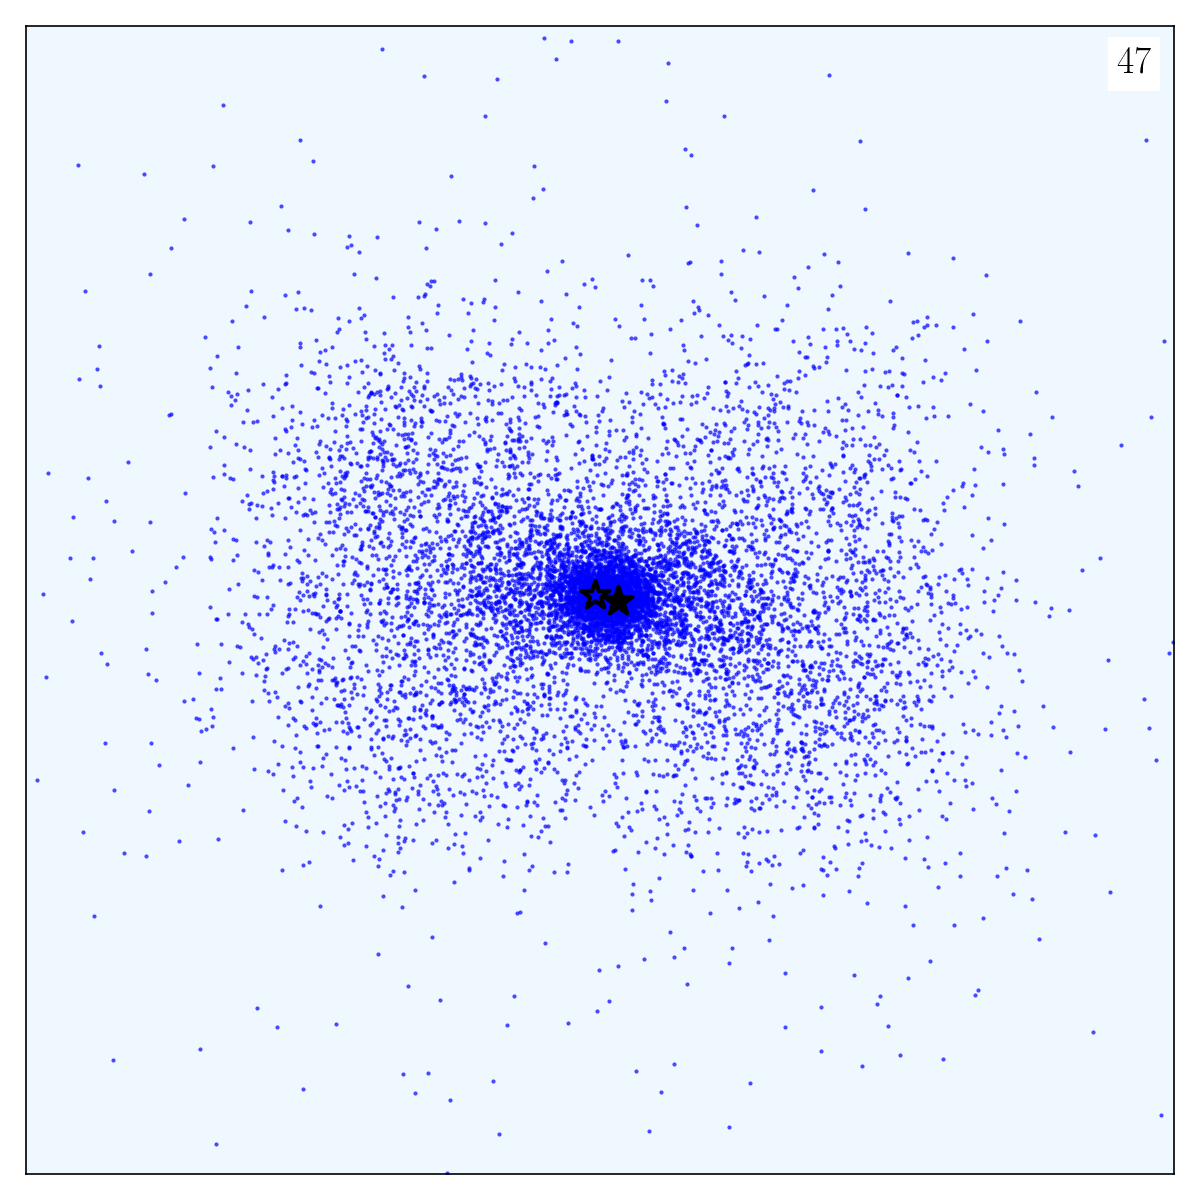
\includegraphics[width = 5.3cm]{images/jumper-demo/particleplot_00047.png}} 	& 
%            {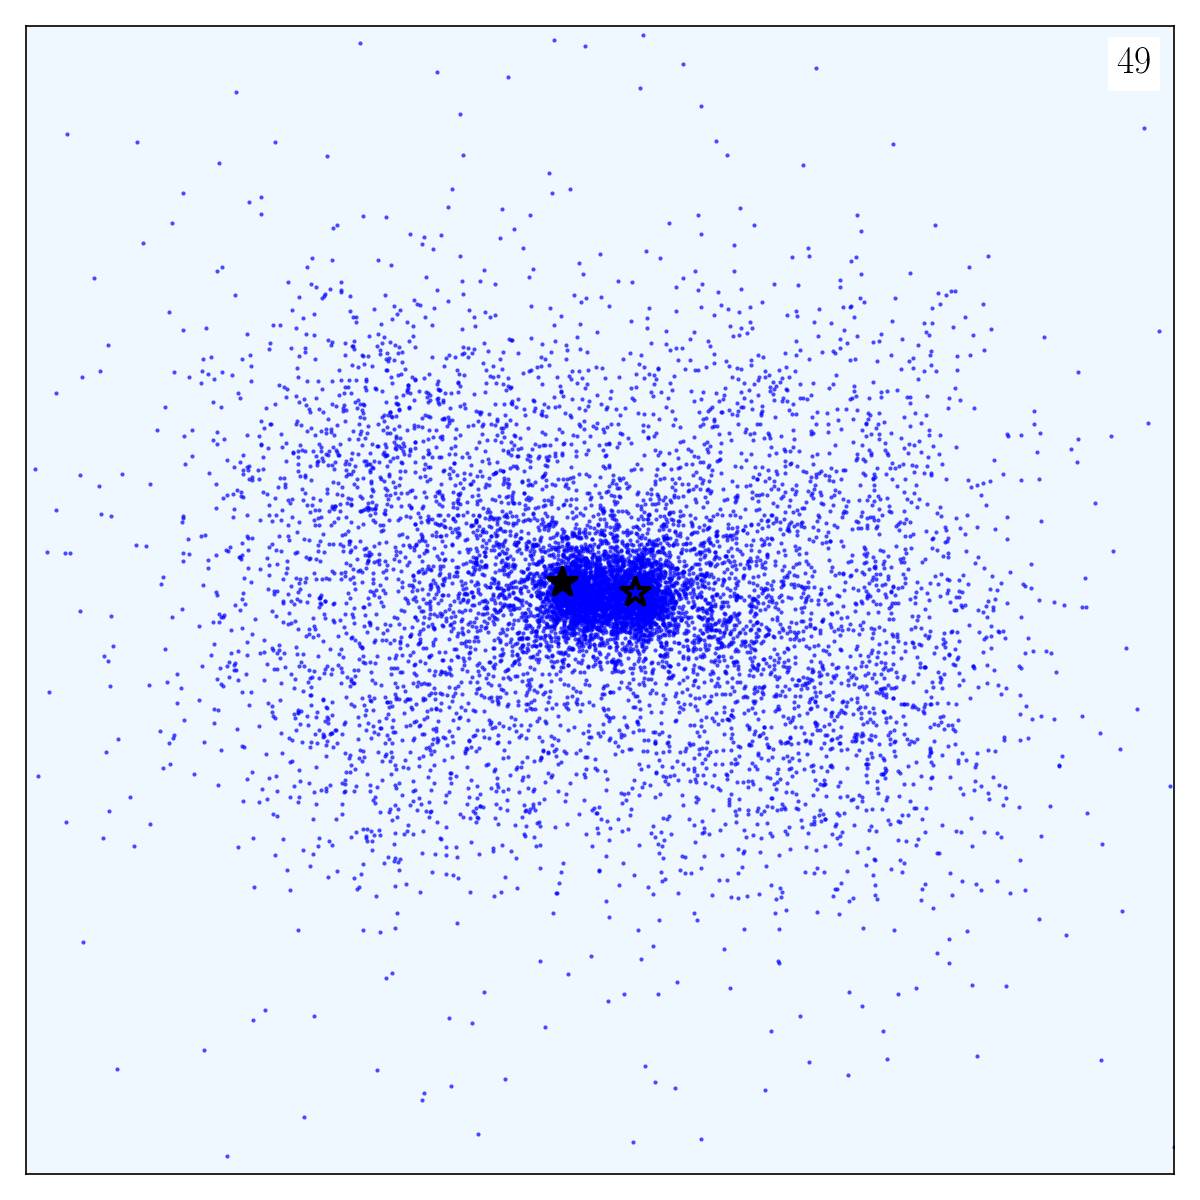
\includegraphics[width = 5.3cm]{images/jumper-demo/particleplot_00049.png}}  \\
        	\hline
    	\end{tabular}
    }
	\caption{\label{fig:jumper-demo} 
        Illustration of how haloes can seemingly merge into another one and re-appear a few snapshots later.
        The green and red particles are two initially distinct haloes that pass through each other.
        The galaxies assigned to them are marked by a star with the same colour as the particles.
        Black stars mark orphan galaxies, which have lost their unique host halo.
        The number in the upper right corner of each plot is the snapshot number that is depicted.
        In snapshots 27-31, the halo-finding algorithm didn't identify both haloes as distinct objects.
        However by tracking the red halo's orphan galaxy, it was possible to link the halo in snapshot 32 all the way back to snapshot 26.\\        
        The simulation was created using \texttt{DICE} \parencite{DICE}.
        Both haloes are identical with mass of $5\cdot 10^{10}\msol$, each containing 5000 particles and following a NFW mass profile.
        The plotted region corresponds to $400$ kpc on each side.
        }
\end{figure}




























































%\begin{sidewaysfigure}[!htbp]
%	{\renewcommand{\arraystretch}{0.1}
%		
%	\subfloat[The results of \phewon\ and \simple\ unbinding of the \ds-dataset: All particles, halo-namegiver particles only and subclumps particles only.]{
%		\begin{tabular}{|p{1cm} c c c|}
%			\hline
%			&&&\\[1em]
%													&
%			\textbf{All particles} 					&
%			\textbf{Halo-namegiver particles only} 	&
%			\textbf{Subhalo particles only} 		\\[1em]
%			%
%			%
%			\begin{sideways}{\hspace{3cm} \phewon}\end{sideways} \hspace*{-1em}%		 
%			& {\includegraphics[width = .28\textwidth]{images/dice-sub/dice-sub-plot-halo1-phew.png}} \hspace*{-1em}%
%			 & {\includegraphics[width = .28\textwidth]{images/dice-sub/dice-sub-halo-only-phew.png}} \hspace*{-1em}% 
%			 &{\includegraphics[width = .28\textwidth]{images/dice-sub/dice-sub-plot-subclumps-phew.png}} \\
%			%
%			%
%			\begin{sideways}{ \hspace{3cm}\simple\ unbinding }\end{sideways}	 \hspace*{-1em}			 &
%			{\includegraphics[width = .28\textwidth]{images/dice-sub/dice-sub-plot-halo1-nosaddle.png}} \hspace*{-1em}&
%			{\includegraphics[width = .28\textwidth]{images/dice-sub/dice-sub-halo-only-nosaddle.png}} \hspace*{-1em}&
%			{\includegraphics[width = .28\textwidth]{images/dice-sub/dice-sub-plot-subclumps-nosaddle.png}} \\
%			\hline
%		\end{tabular}
%		\label{fig:dice_sub_results_a}
%		}
%	}
%	\phantomcaption
%\end{sidewaysfigure}
%%=================================================
%%=================================================
%%=================================================
%\begin{sidewaysfigure}[!htbp]\ContinuedFloat
%	\footnotesize
%	{\renewcommand{\arraystretch}{0.1}
%	\subfloat[The results of \neigh\ and \iter\ unbinding of the \ds-dataset: All particles, halo-namegiver particles only and subclumps particles only.]{
%		\begin{tabular}{|p{1cm} c c c|}
%			\hline
%			&&&\\[1em]
%													&
%			\textbf{All particles} 					&
%			\textbf{Halo-namegiver particles only} 	&
%			\textbf{Subhalo particles only}			\\[1em]
%			%
%			%
%			\begin{sideways}{ \hspace{3cm}\neigh\ unbinding }\end{sideways}		\hspace*{-1em}		 &		
%			{\includegraphics[width = .28\textwidth]{images/dice-sub/dice-sub-plot-halo1-saddle.png}}\hspace*{-1em} &
%			{\includegraphics[width = .28\textwidth]{images/dice-sub/dice-sub-halo-only-saddle.png}}\hspace*{-1em} &
%			{\includegraphics[width = .28\textwidth]{images/dice-sub/dice-sub-plot-subclumps-saddle.png}} \\
%	%		%
%	%		%
%			\begin{sideways}{\hspace{3cm} \iter\ unbinding }\end{sideways}		\hspace*{-1em}		 &		
%			{\includegraphics[width = .28\textwidth]{images/dice-sub/dice-sub-plot-halo1-iter.png}} \hspace*{-1em}&
%			{\includegraphics[width = .28\textwidth]{images/dice-sub/dice-sub-halo-only-iter.png}} \hspace*{-1em}&
%			{\includegraphics[width = .28\textwidth]{images/dice-sub/dice-sub-plot-subclumps-iter.png}} \\
%			%
%			%
%			\hline
%		\end{tabular}
%		\label{fig:dice_sub_results_b}
%		}
%	}
%	\caption{
%	The results of different unbinding methods on the \dt-dataset.
%	}
%	\label{fig:dice_sub_results}
%\end{sidewaysfigure}
%
%